\documentclass[a4paper,12pt]{article}
\usepackage[utf8]{inputenc}

\usepackage[catalan]{babel} % Patrons de trencament de paraula
\usepackage{fancyhdr} % Per la capçalera
\usepackage{geometry}
\usepackage{graphicx} % Per importar logos (i altres gràfics)
\usepackage[colorlinks,linkcolor=black]{hyperref} % Per fer que l'index tingui hiperlinks en el pdf
\usepackage{indentfirst}
\usepackage[sc,small]{titlesec} % Seccions personalitzades

%% Títols
\newcommand{\modulnum}{2}
\newcommand{\modulnom}{Gestió de Bases de Dades}

\newcommand{\ufnum}{1}
\newcommand{\ufnom}{Introducció a les Bases de Dades}

\newcommand{\acttipus}{Pràctica 2}
\newcommand{\actnom}{MasterXef}

%% Entreliniats
\linespread{1.5}

%% Capçalera
\pagestyle{fancy}
\setlength{\headheight}{40pt}
\addtolength{\topmargin}{-20pt}
\fancyhead[L]{\includegraphics*[height=35pt]{provencana_bw.pdf}}
\fancyhead[R]{
	{\scshape\scriptsize Mòdul \modulnum: \modulnom}\\
	{\scshape\footnotesize \acttipus \space  - \actnom}\\
	{\scshape\small Eina Coma Bages i Iris Hidalgo Palomino}}

\addtolength{\textheight}{2cm}

%% Comandes personalitzades
\newcommand{\mygraphic}[2][width=0.9\textwidth]{\begin{center}
		\centering\includegraphics[#1]{#2}\par
\end{center}}

\renewcommand{\contentsname}{Índex}

\begin{document}
\begin{titlepage}
	\centering
	\includegraphics*[width=0.15\textwidth]{provencana_color.pdf}
	\par\vspace{0.5cm}

	{\scshape\Large Institut Provençana \par}

	\vspace{1cm}

	{\itshape\Large \acttipus \par}
	{\bfseries\LARGE \actnom \par}
	
	\vspace{1cm}
	
	{\scshape\large Mòdul \modulnum: \par}
	{\scshape\Large \modulnom \par}

	\vspace{1cm}
	
	{\scshape\normalsize Unitat Formativa \ufnum: \par}
	{\scshape\large \ufnom \par}

	\vfill
	{\Large\itshape Eina Coma Bages \\ Iris Hidalgo Palomino\par}
	\vfill

	Curs 2022/2023
\end{titlepage}

\tableofcontents
\newpage
\section{Diagrama Entitat-Relació}
\begin{center}
	\noindent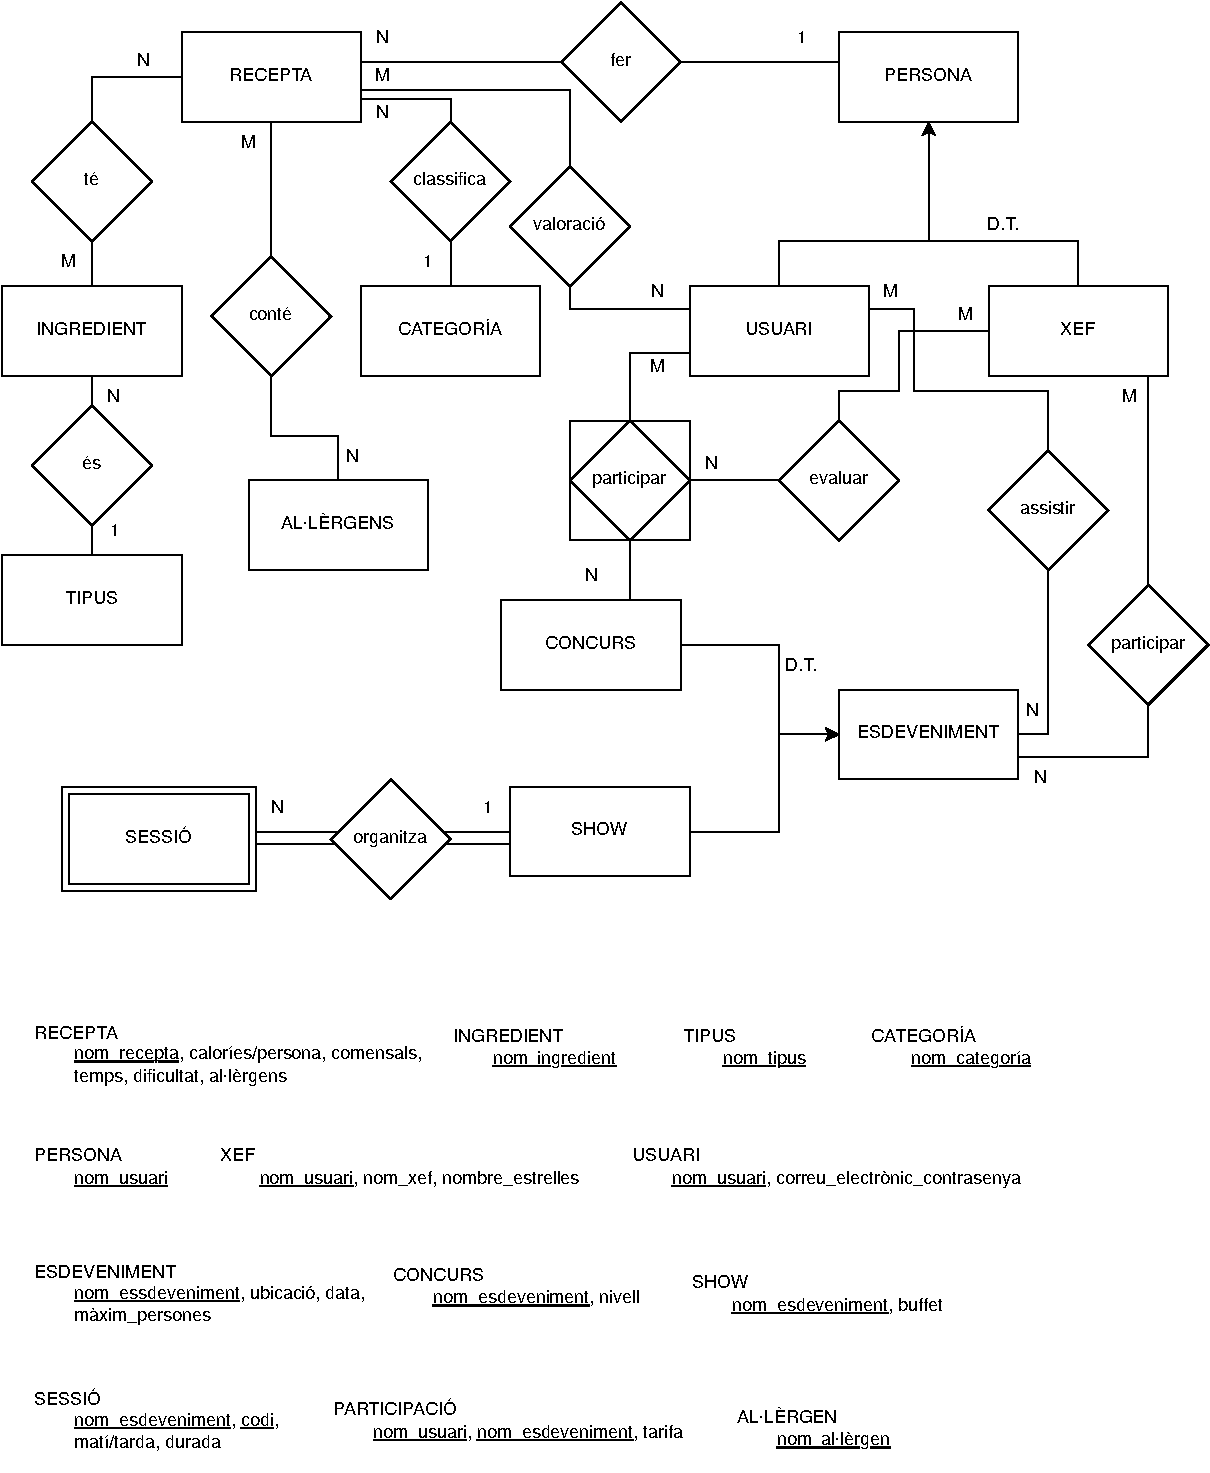
\includegraphics[width=\textwidth]{diagrama.pdf}
\end{center}

\section{Transformació relacional}
\begin{center}
	\noindent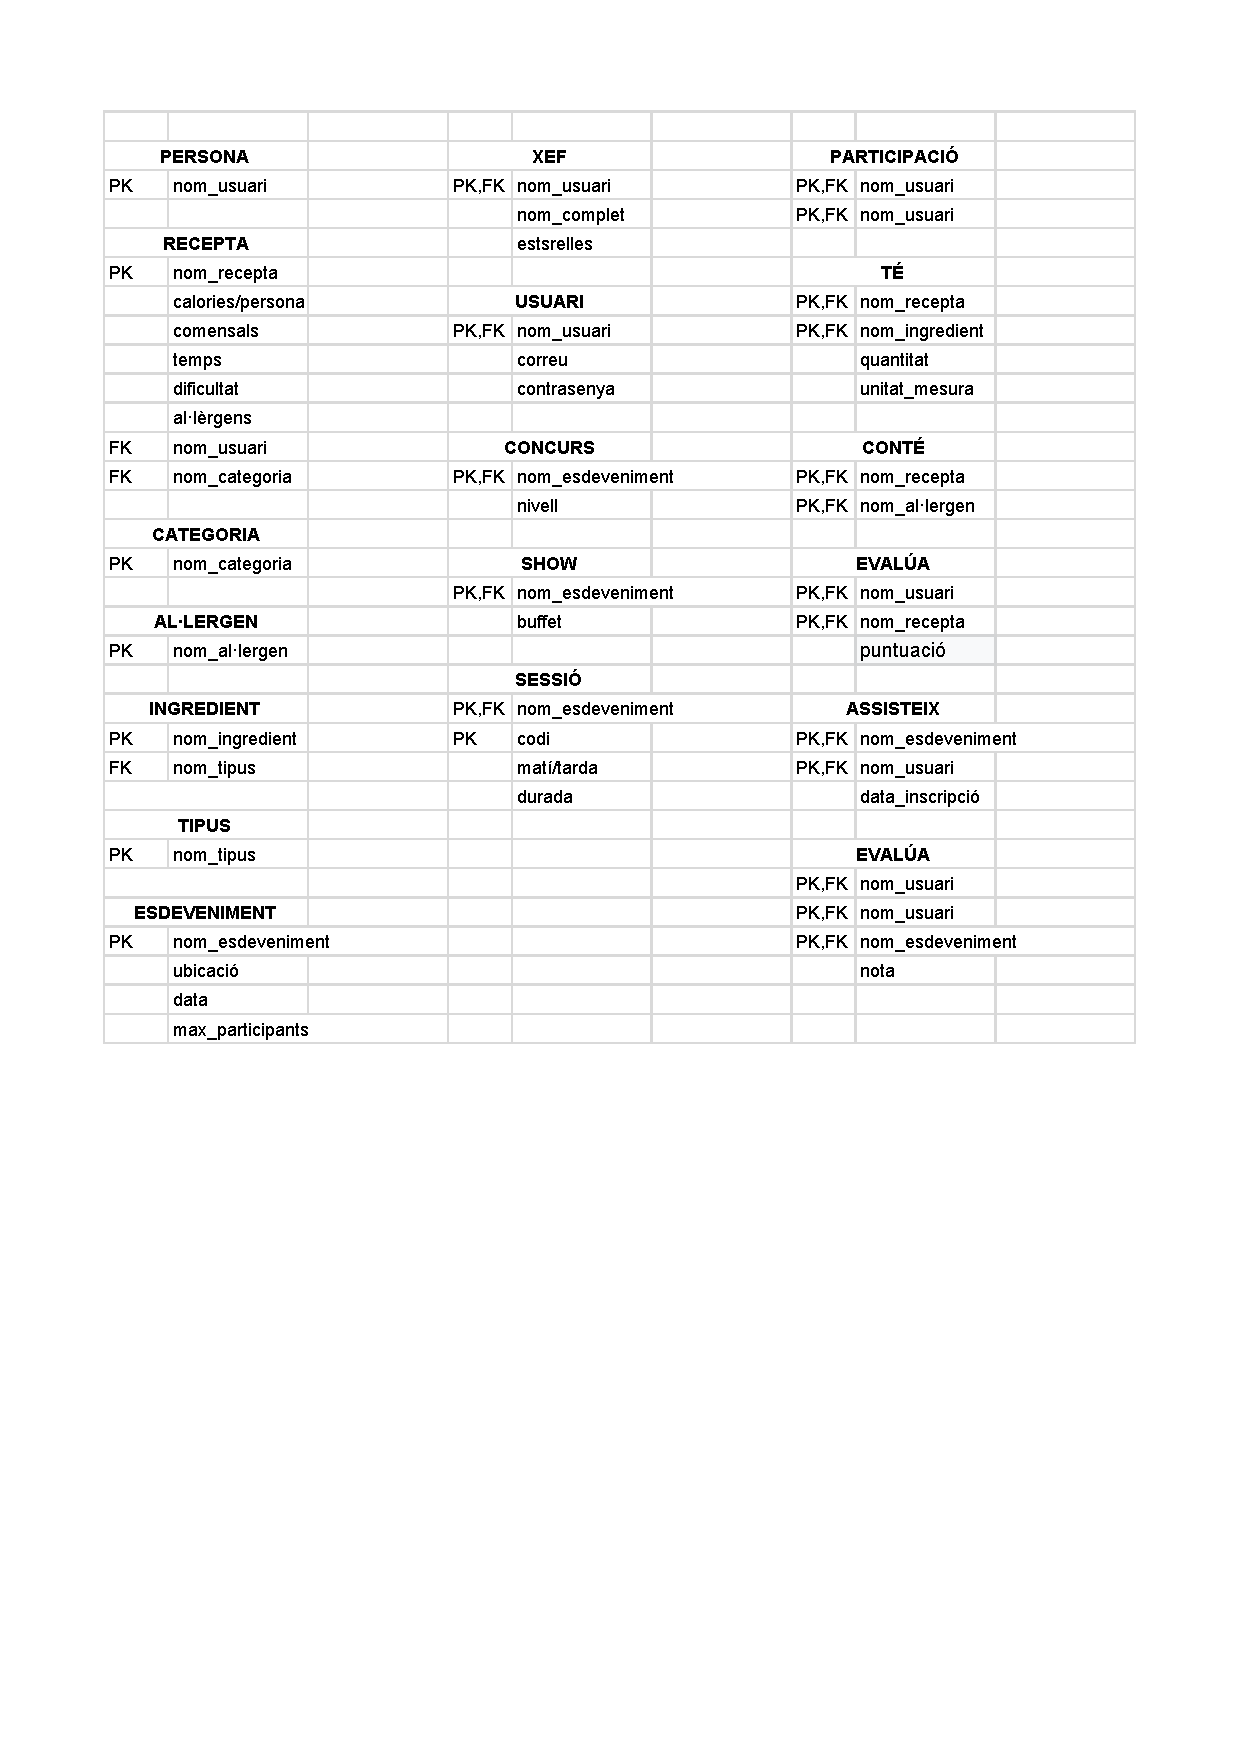
\includegraphics[width=\textwidth]{taula.pdf}
\end{center}

\begin{center}
	\noindent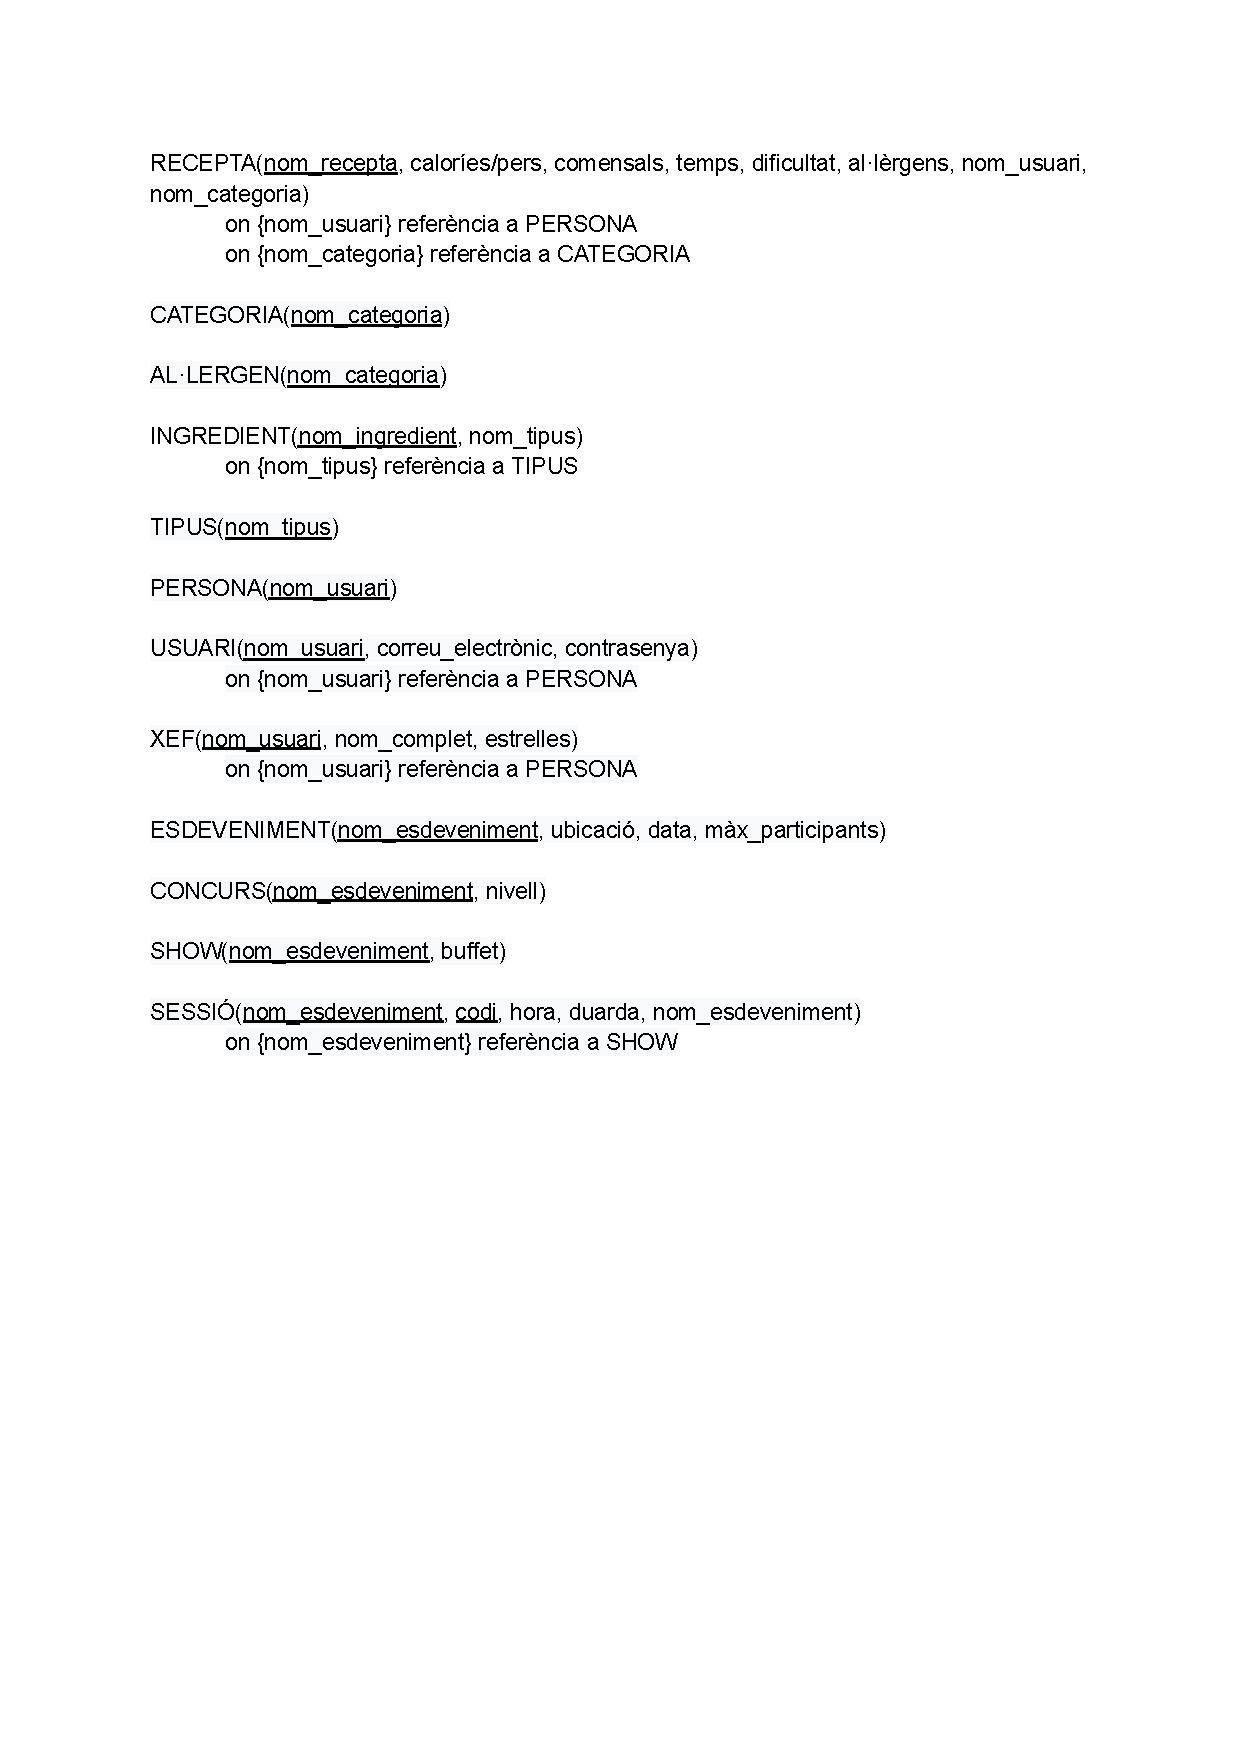
\includegraphics[width=\textwidth]{Model relacional.pdf}
	\noindent\includegraphics[width=\textwidth,page=2]{Model relacional.pdf}
\end{center}

\end{document}